\section{Thesis outline}

\todo{betere openingszin}
All organisms in nature tirelessly perform work, struggling against an ever increasing
entropy. This work is collectively performed by countless molecular machines, all
contributing their specific task.

Most commonly known is the bacterial flagella motor, providing an efficient way for
bacteria to roll and tumble through their environment. The flagella consist of a
stator connected to the cell membrane and a rotor providing the rotary motion. The
work is produced by the flow of cations through the stator, inducing changes in the
electrostatic interactions between the two parts of the flagella, generating
unidirectional motion.\\

Whilst being so abundantly present in nature, fabricating synthetic molecular machines
turns out to be a difficult task.
One of the biggest hurdles in this process arises from the length-scale of these
machines. Often times not these structures are not larger then a few nanometres, making
the dominant forces result from random thermal fluctuations. These stochastic forces
result in the Brownian motion of these molecular machines. Using these random motion no
usefeull work can be extracted, to overcome this hurdle often time synthetic molecular
machines are embeded in surfaces like bilipid layers.

%No work can be extracted from freely tumbling, randomly oriented molecules.  This
%fundemental limit has been overcome by interfacing synthetic molecular machines
%with surfaces.\\




dissipating heat, soft large structures.  polymers, DNA.

DNA piston can be characterised as a autonomous molecular machine, which turns
over chemical fuel to perform work continuously. bayoumi et al.

aim of the molecular machine is to perform selective transport of dna through the
membrane. This has been done before following an external bias, but special is that the
machine opperates also opposing a external bias. The physics that makes this special
property possible is entropy and will be discussed futher in detail in later chapters of
this thesis.

thesis outline, first chapter is a short introduction to important concepts. chapter two
is a discussion of the dna nanopiston, largely based on the paper recently published by
bayoumi et al. Next adaptation of the model is discussed in chapter 3. The results of
these simulations are discussed in the last chapter.

\begin{figure}
\begin{center}
  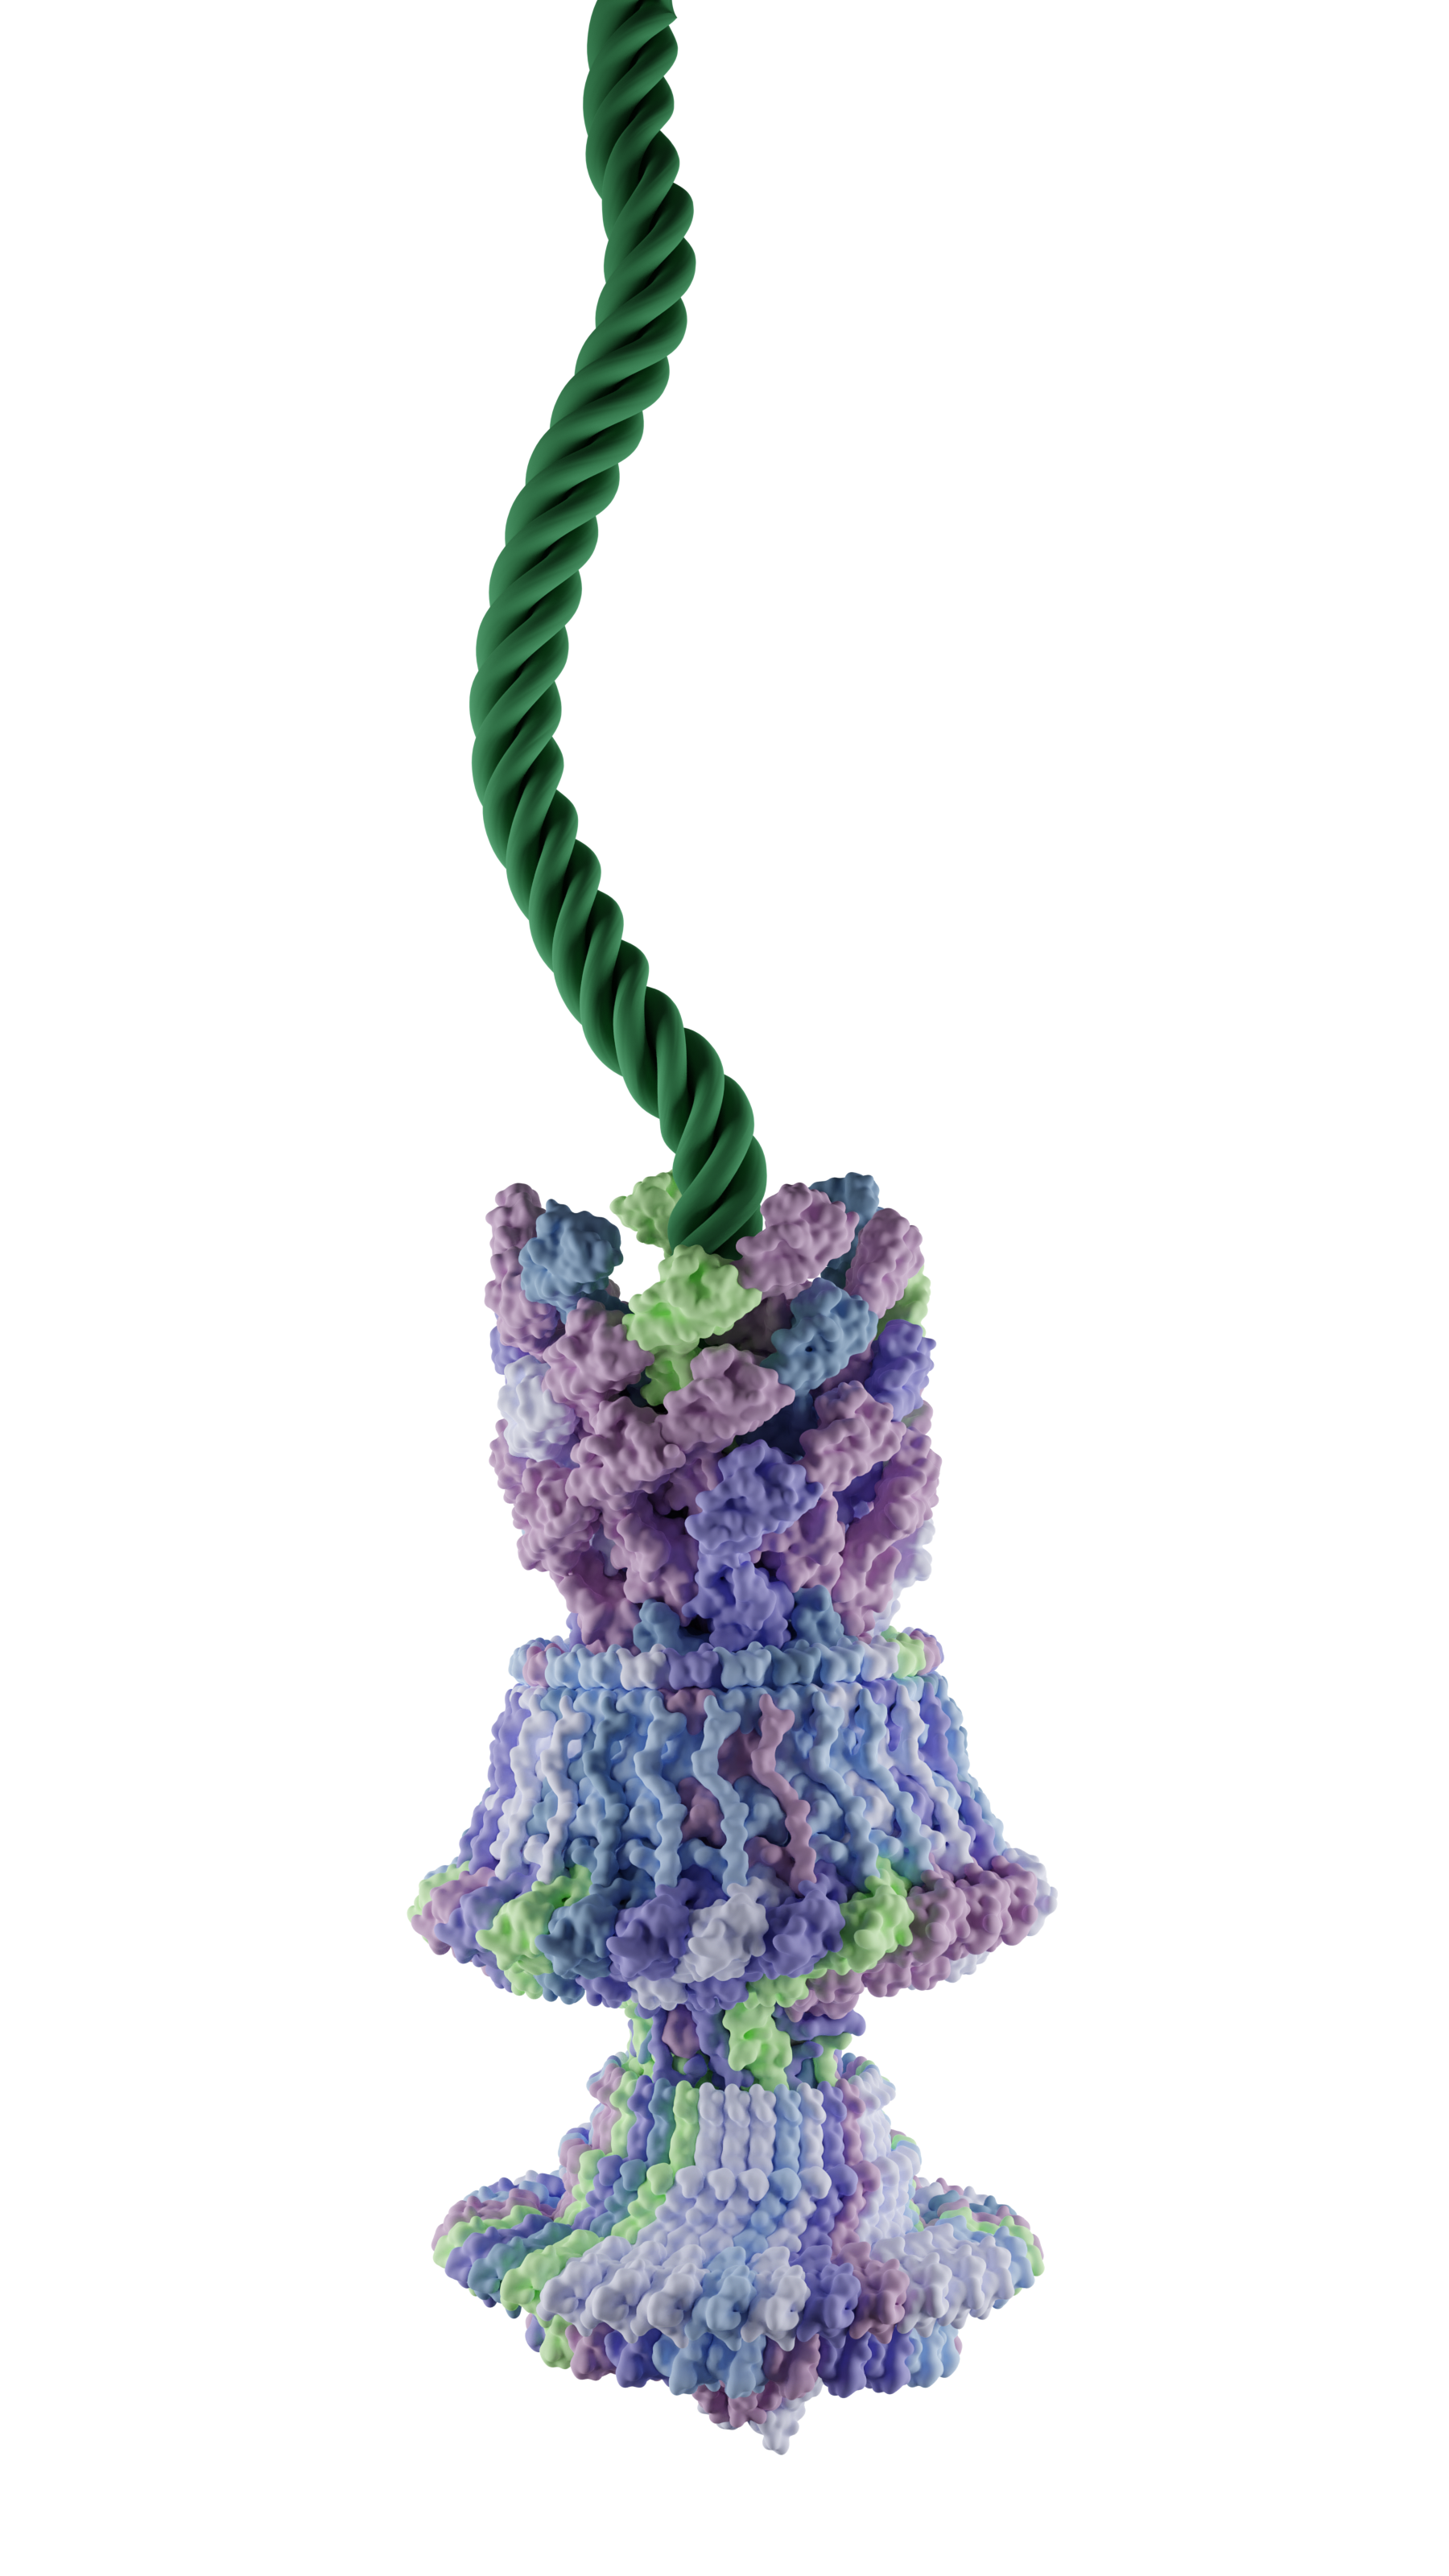
\includegraphics[width=0.80\textwidth]{Figures/flagella.png}
  \caption{write caption}
\end{center}
\end{figure}
